\documentclass[11pt]{article}
\usepackage[a4paper,margin=25mm]{geometry}
\usepackage{amsmath,amssymb,booktabs,graphicx,hyperref,microtype}
\graphicspath{{../figures/}}
\title{Finite Chebyshev-Tail Diagnostics and Symmetry Orbits: A Reproducible Research Module}
\author{Shanti Draconis\\\small Draft research artefact}
\date{5 August 2026}
\begin{document}
\maketitle

\begin{abstract}
We provide a reproducible finite computation module for the Chebyshev function
$\psi(x)=\sum_{p^k\le x}\log p$ and the residual $E(x)=\psi(x)-x$.  The
module visualizes finite tail data, a windowed amplitude diagnostic, and the
symmetry orbit of a hypothetical off-critical zeta zero.  Its purpose is to
make the distinction between an experimental signal, an exact finite identity,
and a global mathematical conclusion machine-readable.  It does not prove or
disprove the Riemann Hypothesis.
\end{abstract}

\section{Scope}
The Riemann Hypothesis is the statement that every nontrivial zero $\rho$ of
$\zeta(s)$ has $\Re(\rho)=1/2$.  Finite computation can test inputs and
produce candidate phenomena; it cannot establish this universal statement.
The Euler product is not used as a convergent expression in the critical strip.

\section{Tail diagnostic}
For integer $x\ge2$, define
\[
 \psi(x)=\sum_{p^k\le x}\log p,\qquad E(x)=\psi(x)-x.
\]
The explicit formula motivates studying $E$, but the implementation computes
$\psi$ directly from prime powers.  To avoid interpreting isolated sign changes
as exponents, we report a windowed normalized energy
\[
 \mathcal E_h(U)=\left(\frac1h\int_U^{U+h}
 \left|e^{-u/2}E(e^u)\right|^2\,du\right)^{1/2},
\]
approximated on a finite grid.  This is a diagnostic definition, not an
estimator proved consistent for the supremum of real parts of zeta zeros.

\section{Symmetry orbit}
For a hypothetical generic zero $\rho=\sigma+it$ off the critical line, the
functional equation and conjugation imply the orbit
\[
 \{\rho,\overline\rho,1-\rho,1-\overline\rho\}.
\]
This is a finite symmetry orbit.  It does not imply an infinite family of zeros
off the line, nor does it provide a trajectory to the trivial zeros.

\section{Control example}
The Fibonacci recurrence has the exact Binet decomposition
\[
 F_n=(\varphi^n-\widehat\varphi^n)/\sqrt5.
\]
Its normalized ratio error is an exactly solved, exponentially decaying control.
It validates the implementation of a tail-style plot; it transfers no theorem
to the zeta function.

\section{Reproducibility and limitations}
The script records the integer range, sample grid, and output CSV.  All figures
are labelled as finite diagnostics.  A proof of RH would require a valid global
argument controlling all nontrivial zeros; this module supplies none.

\begin{figure}[ht]
\centering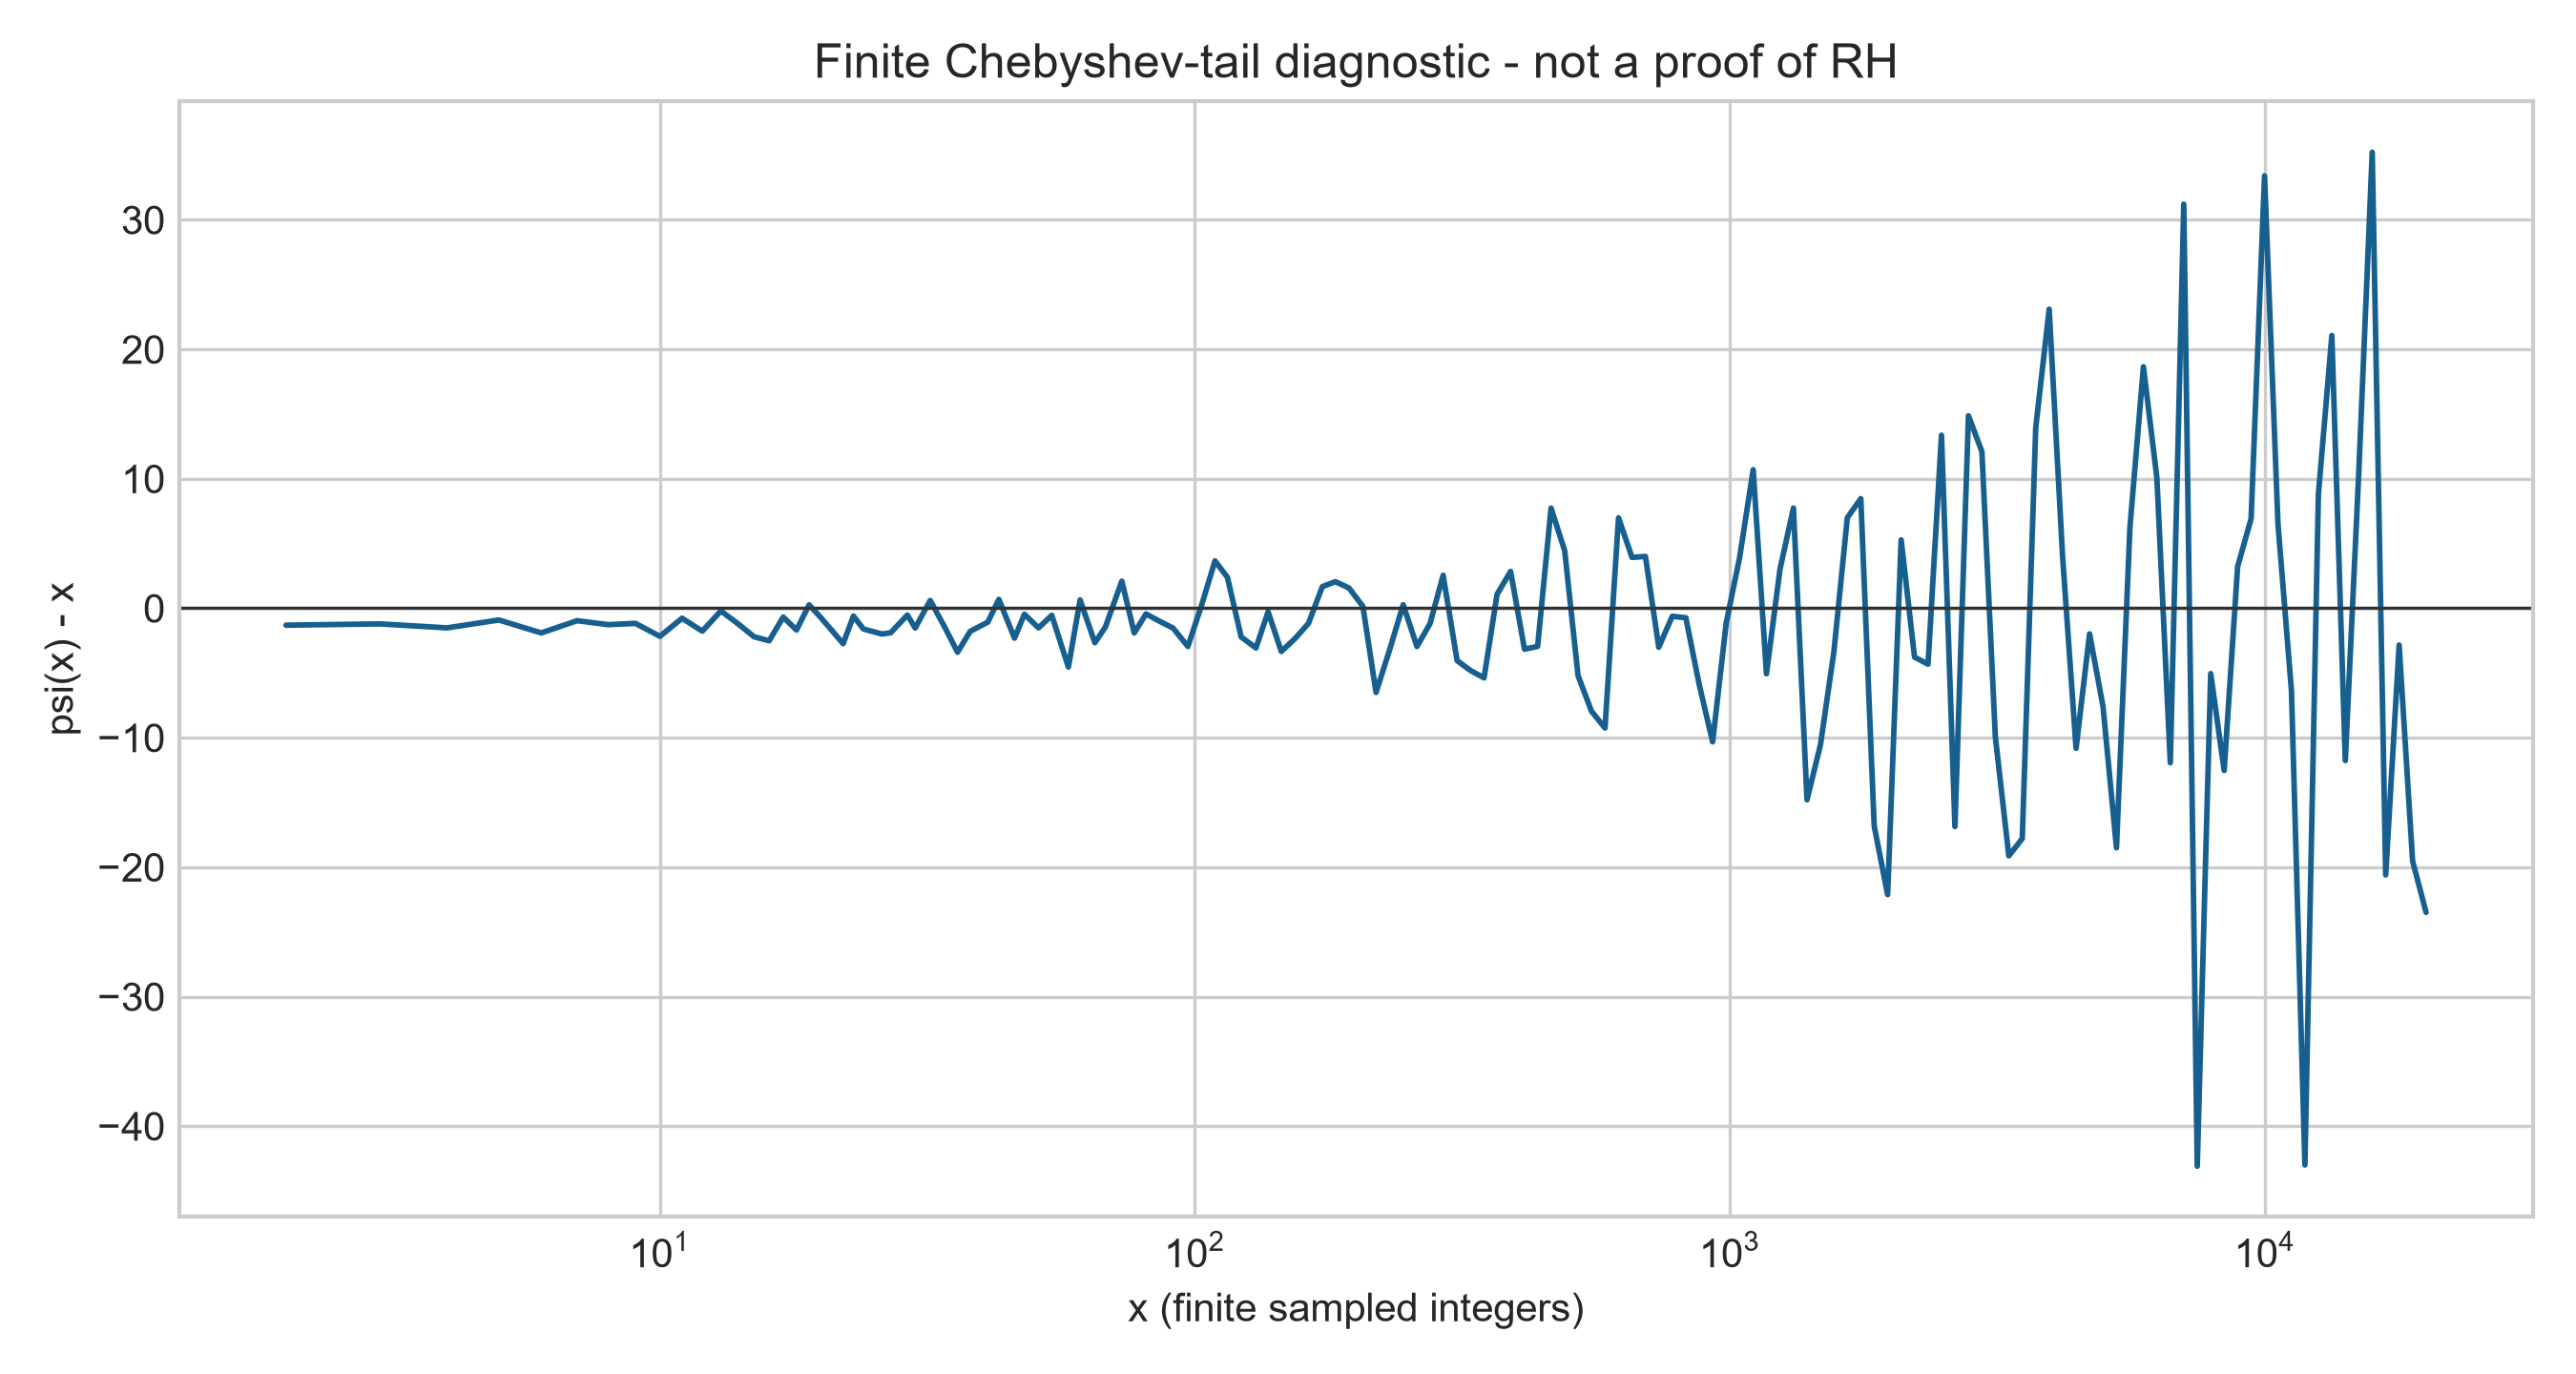
\includegraphics[width=.9\linewidth]{chebyshev_tail.png}
\caption{Finite values of $E(x)=\psi(x)-x$.  The plot is numerical evidence
over the selected range, not a bound for all $x$.}
\end{figure}

\begin{figure}[ht]
\centering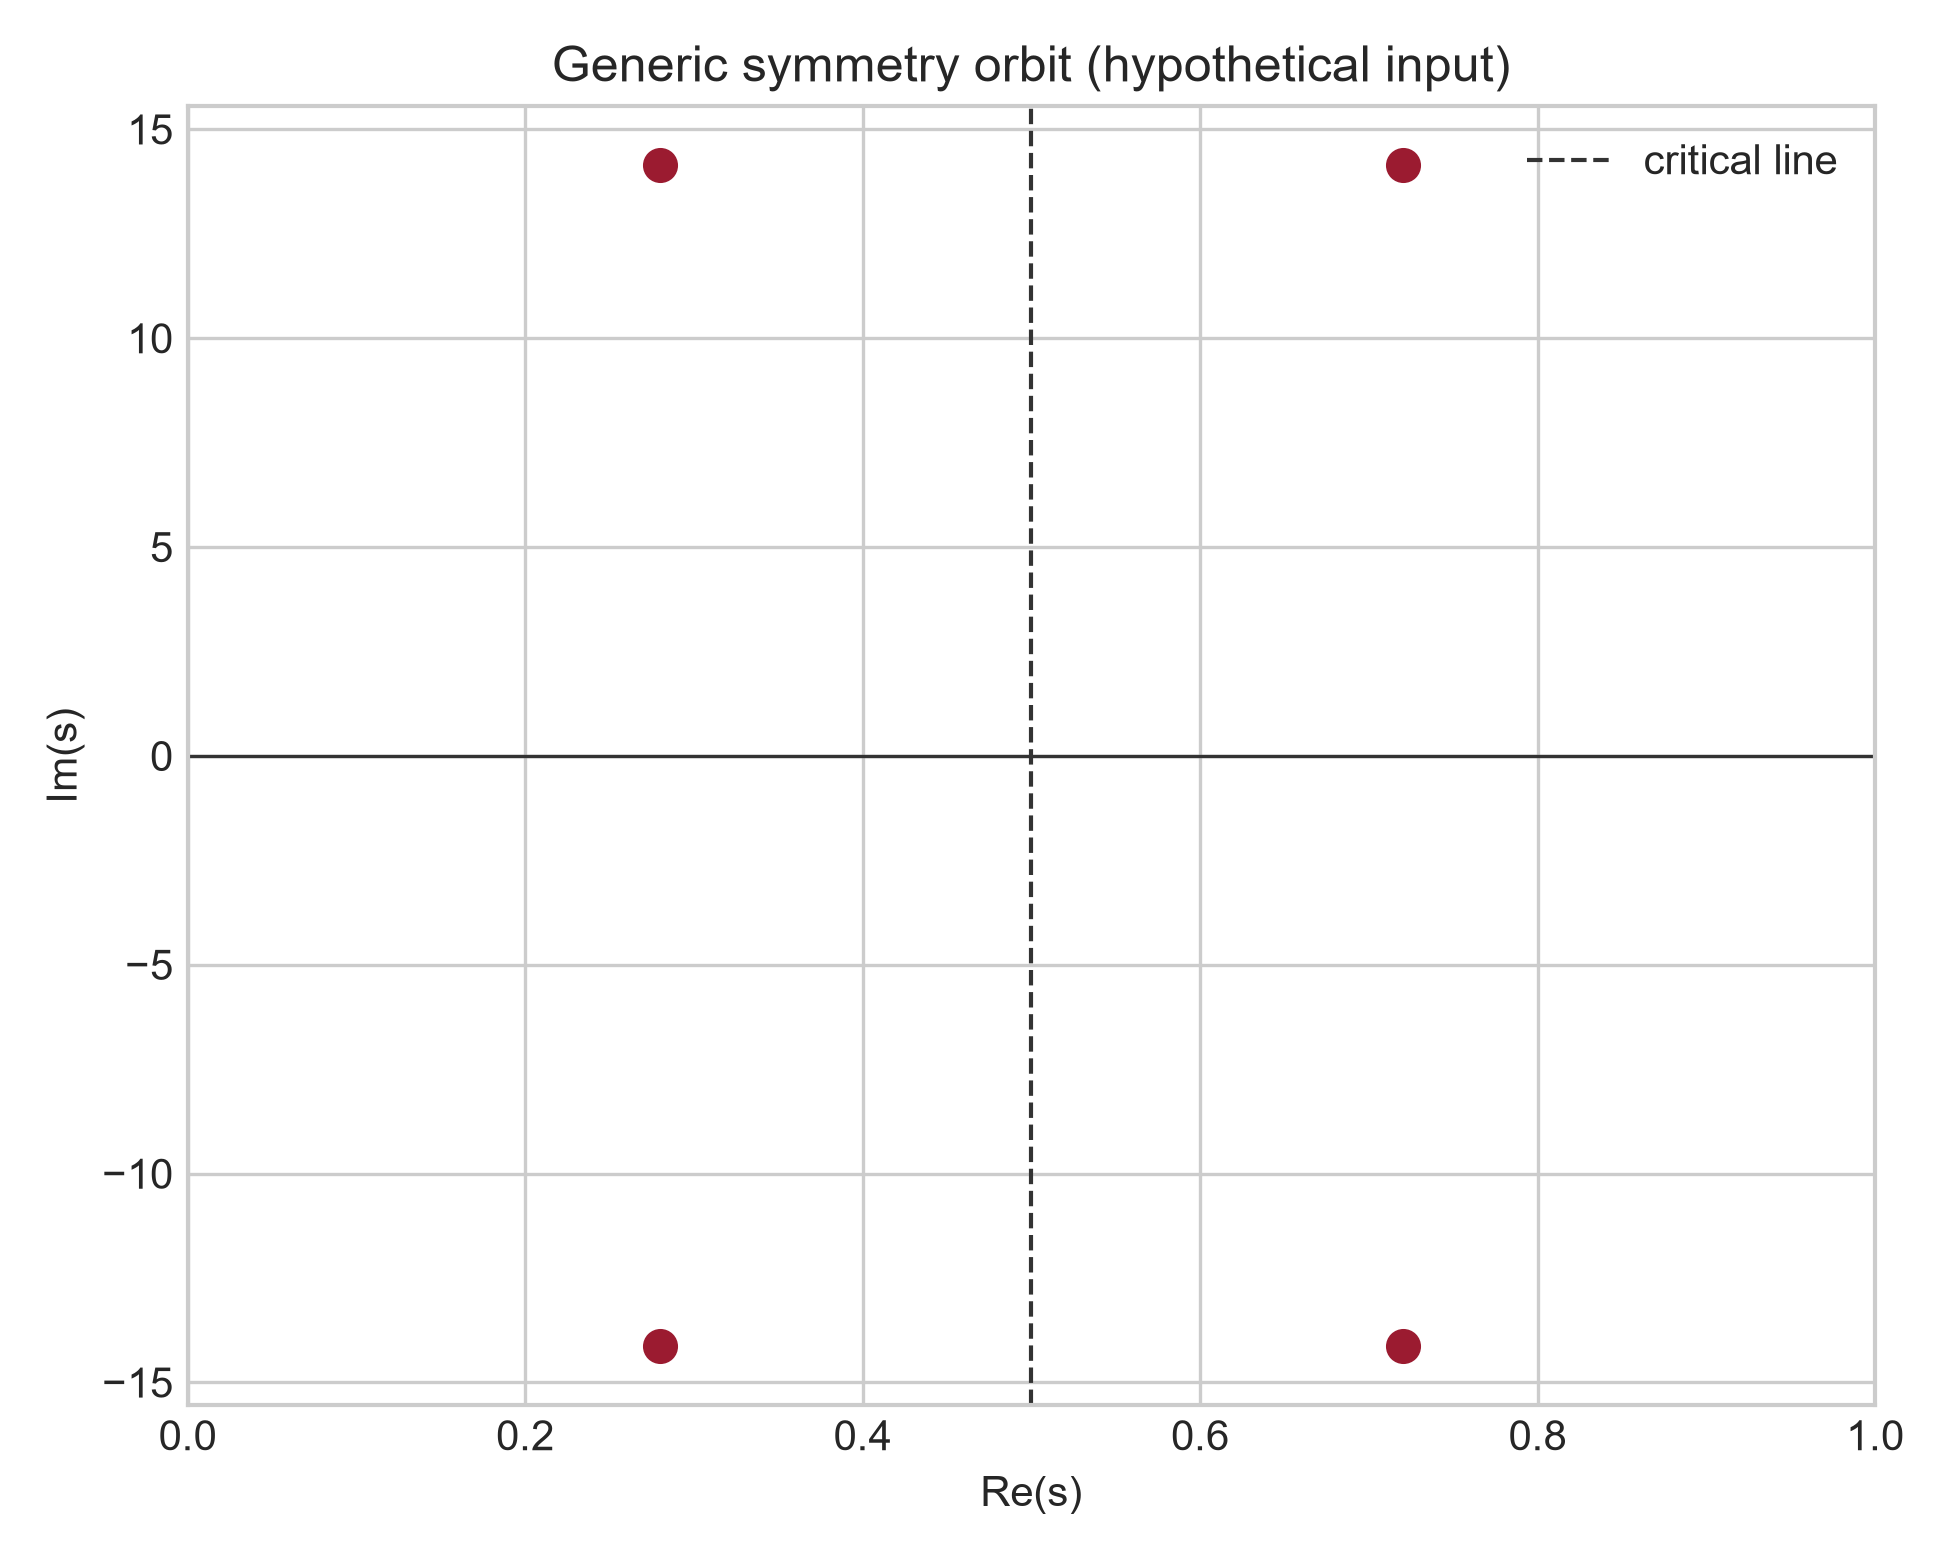
\includegraphics[width=.72\linewidth]{zero_orbit_geometry.png}
\caption{Generic fourfold symmetry orbit for a hypothetical off-critical
zero.  This is geometry of the functional-equation symmetry, not observed data.}
\end{figure}

\bibliographystyle{plain}
\begin{thebibliography}{9}
\bibitem{dlmf} NIST Digital Library of Mathematical Functions, Chapter 25,
\emph{Zeta and Related Functions}, \url{https://dlmf.nist.gov/25.16}.
\bibitem{bombieri} E. Bombieri, \emph{Problems of the Millennium: The Riemann
Hypothesis}, Clay Mathematics Institute, 2000.
\end{thebibliography}
\end{document}
